\chapter{Ocenjevanje in izbor atributov}

Ocenjevanje in izbor atributov sta osnovni opravili vsakega podatkovnega rudarja. Namreč, odkrivanje znanj iz podatkov temelji na tem, da ugotovimo, kateri atributi pomembni in prevladujoče vplivajo na obnašanje modela, kakršenkoli naj slednji bo. V tem poglavju se bomo sicer s primerom omejili na klasifikacijske probleme, a je koncepte, ki jih bomo spoznali, prav enostavno razširiti na kakršenkoli drugo nalogo.

Ocenjevanje informativnosti atributov je predvsem pomembno takrat, ko želimo podatke in iz teh porajajoče se modele razumeti. Na primer, želimo vedeti, kateri od atributov, s katerim opišemo naročnika mobilnih storitev, je tisti, ki je najbolj povezan z prekinitvijo naročniškega razmerja. Ali pa, v medicini, kateri od simptomov je najbolj povezan z diagnozo, ali pa prognozo. Morda celo, katere so tiste ključne besede v čivkih, ki so povezane s tečajem določene valute.

Z ocenjevanjem informativnosti atributov je povezan tudi njihov izbor. V splošnem bi iz začetne množice atributov, s katerimi smo popisali primere, radi izbrali množico atributov, ki je po nekem kriteriju najboljša. Recimo tako, na podlage katere nam izbrana metoda strojnega učenja zgradi model z visoko napovedno točnostjo. Na podlagi stopnje povezanosti oziroma vključenosti ocenjevanja v izgradnjo modelov tudi ločimo tri različne načine izbora atributov:
%
\begin{enumerate}
\item {\bf Filter}. Atributom pripišemo stopnjo informativnosti, ki jo izračunamo neposredno iz podatkov. Pri tem lahko upoštevamo samo vrednosti atributa in razreda (univariatni pristop) ali pa kontekst, torej tudi vrednosti ostalih atributov (multivariatni pristop). Predvsem univariatne metode so lahko izjemno časovno učinkovite, a je tu težava pri določanju praga, koliko atributov izbrati. Kratkovidnost univariatnih metod rešujemo z multivariatnimi pristopi (npr. metoda Relief), ki pa so časovno potratnejše. Tudi pri njih ostaja problem, koliko atributov izbrati.
\item {\bf Ovojnica}. Atribute izberemo tako, da optimiziramo napovedno točnost modelov. Tipično zberemo neko začetno množico atributov, preverimo napovedno točnost modela, ki ga zgradimo na tej množici, in tej množici dodajamo ali odvzemamo atribute s ciljem izboljšanja točnosti. Metode te vrste so tipično časovno potratne.
\item {\bf Metoda učenja.} Veliko metod strojnega učenja z uteževanjem ali kar neposredno z uporabo samo nekaterih atributov na ta način, torej znotraj metode, vrši izbor značilk. Primer takih tehnik so regresijska in klasifikacijsko drevesa, naključni gozdovi ter linearna in logistična regresija. Pri slednjih je še posebej zanimiva kombinacija z regularizacijo L1.
\end{enumerate}

Obstaja vrsta odličnih pregledov različnih vrst in tipov zgoraj omenjenih metod. Cilj tega poglavja je samo osnovni pregled, morda še ožje, relacija med izborom značilk in nevarnostjo, da se z njo preveč prilagodimo podatkom. A pojdimo po vrsti in pričnimo s primerom.

\section{Primer podatkov}

Za primer si poglejmo podatke, iz katerih lahko morda ugotovimo, ali ima kajenje sploh kakšne posledice. Recimo, na [limfocite](https://sl.wikipedia.org/wiki/Limfocit), to je na vrsto belih krvnih telesc. Še najbolj sistematično lahko posledice kajenja opazujemo tako, da pogledamo, kaj se dogaja v celicah limfocitov. Biologi danes dogajanja v celicah opazujejo tudi preko izražanja vseh genov v celici (človekov genom jih ima okoli $20.000$). To je, z meritvami, koliko so geni aktivni pri proizvajanju proteinov. Še bolj direktno bi stanje v celici lahko ocenili s koncentracijo vseh proteinov, a je ta tehnologija dražja in manj dostopna. Tu nas je morda malce zaneslo pri domeni vsled piščeve navdušenosti nad biotehnolgoijo, ampak na koncu je enostavno: imamo primere (79 žensk, med njimi 40 kadilk in 39 nekadilk) in meritve izražanj $14.093$ genov v njihovih limfocitih (atributi). Podatki so prosto dostopni v zbirki GEO Data Sets~\footnote{\url{https://www.ncbi.nlm.nih.gov/sites/GDSbrowser?acc=GDS3713}}. Naš cilj je ugotoviti, koliko atributov nam pove kaj o razredu. Oziroma, po biološko, koliko je takih genov, katerih izražanje se spremeni pri kadilkah.

\section{Ocenjevanje informativnosti}

Pod informativnost tu razumemo povezanost med vrednostjo atributa in razredom. Z drugimi besedami, v kakšni meri lahko iz vrednosti atributa napovemo razred. Kot kaže slika~\ref{f:fss-instance-dist}, so lahko atributi bolj ali manj povezani z razredom.

\begin{figure}[htbp]
\centering{
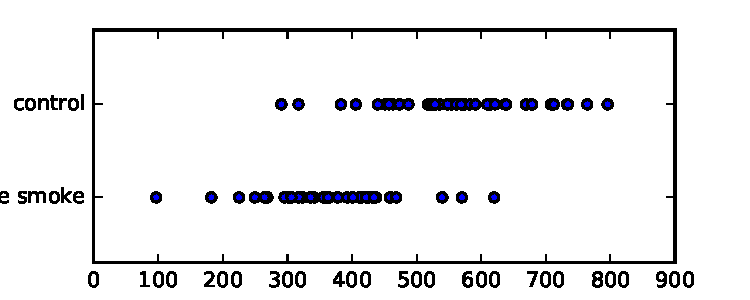
\includegraphics[width=10cm]{slike/fss-informative.pdf}
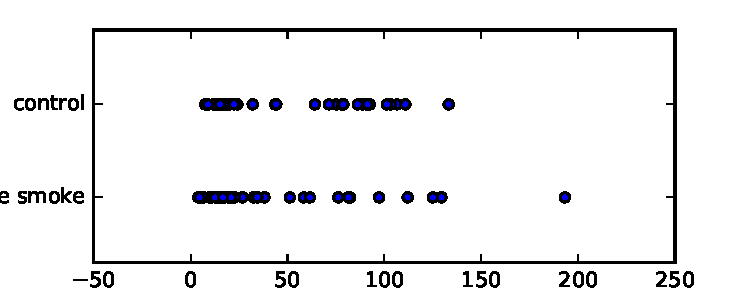
\includegraphics[width=10cm]{slike/fss-noninformative.pdf}
\caption{Porazdelitev vrednosti informativnega (zgoraj) in neinformativnega (spodaj) atributa pri primerih v prvem (``control'') in drugem razredu (``cigarette smoke'').}
\label{f:fss-instance-dist}}
\end{figure}

Pri zveznih atributih in diskretnem razredu za informativen atribut pričakujemo, da bo ta zavzel podobne vrednosti pri primerih istega razreda, ki bodo drugačne od vrednosti atributov za primere ostalih razredov. Za binarno klasifikacijo nam to razliko dobro kvantificira Studentovo t-statistika za ocenjevanje razlik med dvema skupinama meritev $X_0$ in $X_1$, kjer so v matriki $X_0$ zapisane atributne vrednosti primerov enega razreda ($y=0$) in v matriki $X_1$ atributne vrednosti primerov drugega razreda ($y=1$). Želimo torej, da bi bila povprečna vrednost med tema skupinama čim bolj drugačna, torej absolutna razlika med njima čim večja, ter da bi razsipanje vrednosti znotraj skupin bilo čim manjše. Pri slednjem bi bilo dobro upoštevati tudi število primerov v posamezni skupine. Vse skupaj strnemo v enačbo za že omenjeno t-statistiko:

$$t=\frac{\mean{X_0}-\mean{X_1}}{\sqrt{\ds\frac{s_0^2}{n_0}+\frac{s_1^2}{n_1}}}$$

kjer sta $s_0$ in $s_1$ standardna odklona vzorcev $X_0$ in $X_1$. Zanima nas povprečna vrednost t-statistike, torej $|t|$. Za naš primer kadilk in nekadilk je porazdelitev vrednosti te statistke, torej vrednosti ocen informativnosti atributov takšna, kot jo prikazuje slika~\ref{f:fss-score-dist-true}.

\begin{figure}[htbp]
\centering{
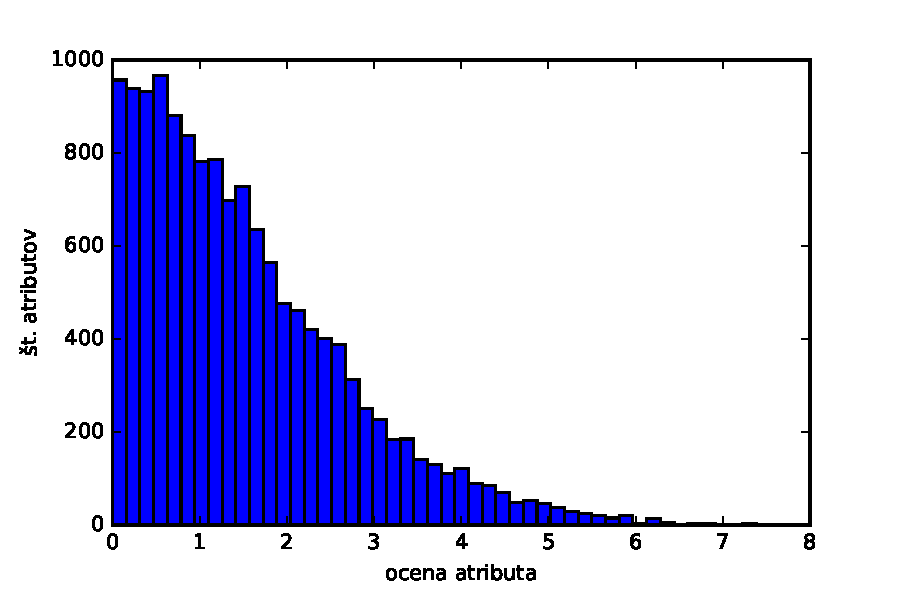
\includegraphics[width=10cm]{slike/fss-score-dist-true.pdf}
\caption{Porazdelitev ocen informativnosti atributov.}
\label{f:fss-score-dist-true}}
\end{figure}

Tu je na mestu opozorilo. Zgoraj smo uvedli eno od metod za univariatno ocenjevanje informativnosti atributov. Ta je priročna samo v primeru, ko je atribut zvezen, razred pa binaren. V primeru večvrednostnega razreda bi bilo potrebno uporabiti statistiko ANOVA. Če bi bili atributi diskretni, bi lahko uporabili informacijski prispevek, ali pa $\chi^2$. Univariantnih za različne kombinacije tipov atributov in razredov je veliko in bi bilo naštevanje na tem mestu neprimerno enciklopedično. Raje nadaljujmo z vprašanjem, kaj nam sploh ocene atributov povedo oziroma kateri atributi so potem sploh povezani z razredom. Ali bolje, kje, na sliki~\ref{f:fss-score-dist-true} je meja, od katere naprej bi lahko trdili, da je atribut informativen.

\section{Permutacijski test}

Naši podatki vsebujejo veliko število atributov in relativno majhno število primerov. Prav lahko bi se zgodilo, da je kakšen od teh atributov informativen popolnoma naključno, torej, da so meritve bile slučajno take, da so ravno dovolj ločile izbrani dve skupini oziroma razreda. Kakšna bi bila potem porazdelitev atributnih ocen, torej porazdelitev, če bi bile meritve naključne meritvah? Ali pa, če bi laborant pomešal oznake vzorcev in bi bili razredi primerov napačni. Do naključnih meritev lahko pridemo tako, da vrednosti za dani atribut premešamo, še lažje pa to storimo za vse atribute naenkrat tako, da premešamo vrednosti razredne spremenljivke. Po tej permutaciji ocenimo informativnost atributov. Da vse skupaj ne bo odvisno od ene same permutacije razredov, lahko postopek nekajkrat ponovimo. Za naše podatke in oceno s t-statistiko dobimo porazdelitev ocen, kot nam jo prikazuje graf na sliki~\ref{f:fss-score-dist-null}.

\begin{figure}[htbp]
\centering{
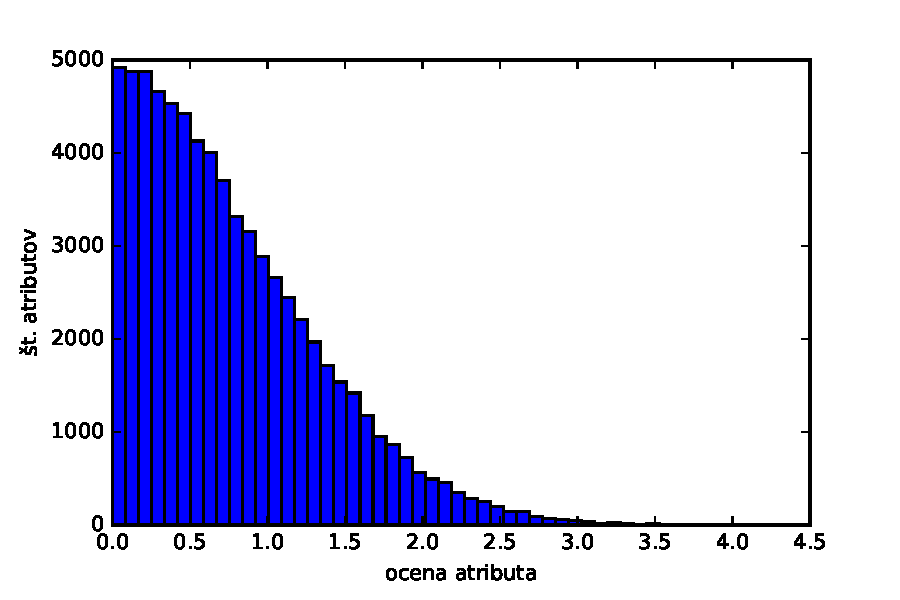
\includegraphics[width=10cm]{slike/fss-score-dist-null.pdf}
\caption{Porazdelitev ocen informativnosti atributov, ki smo jih dobili na ``pokvarjenih'' podatkih, kjer smo premešali vrednosti razredne spremenljivke oziroma premetali kolono z razredom.}
\label{f:fss-score-dist-null}}
\end{figure}

Porazdelitev ocen informativnosti atributov, ki jih izračunamo nad ponaključenimi podatki, je dosti ožja od te pridobljene iz originalnih, ``nepokvarjenih'' podatkov. Slika~\ref{f:fss-score-dist-both} nam prikazuje obe distribuciji hkrati. Na njej smo z navpično nakazali na mejo, od katere dalje je na permutiranih podatkih zelo majhno število ocen oziroma je delež takih meritev samo $p=0.001$. Za vse atribute, ki so bili ocenjeni desno od te meje, lahko trdimo, da je vrednost njihove ocene taka, da bi jo težko dobili na naključnih podatkih. Verjetnost, da bi se to lahko zgodilo, je enaka vrednosti $p$, na podlagi katere smo mejo določili. Če bi radi to verjetnost še zmanjšali, ustrezno zmanjšamo vrednost $p$. Koliko je sploh takih atributov? Za našo izbrano vrednost meje oziroma napake $p$ je takih 1327 atributov, se pravi, nekako desetina vseh genov, ki so bili vključeni v meritve. Pri veliko strožji meji, na primer $p=0.0001$, se število takih atributov zmanjša na 734.

\begin{figure}[htbp]
\centering{
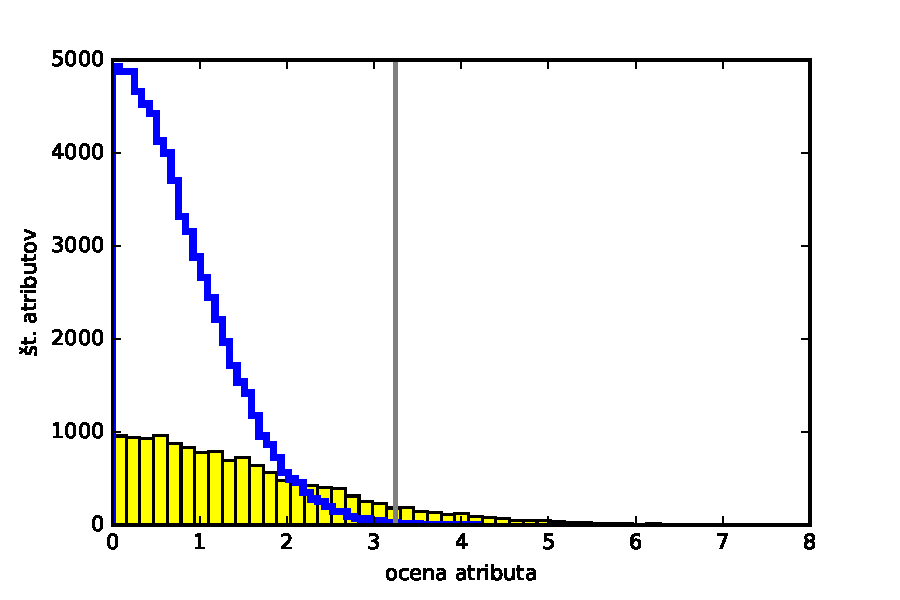
\includegraphics[width=10cm]{slike/fss-score-dist-both.pdf}
\caption{Primerjave porazdelitve ocen informativnosti atributov na ponaključenih podatkih (rumena črta) in pravih podatkih (histogram v modrem).
Siva navpičnica nakazuje mejo, od katere desno je samo zelo majhen delež ocen ($p=0.001$), ki so bile pridobljene na naključnih podatkih. 
}
\label{f:fss-score-dist-both}}
\end{figure}

V podatkih je torej samo približno desetina atributov, za katere kaže, da so povezani z razredom. To je pravzaprav za naš problem zelo veliko. Spomnimo se, preučujemo učinke kajenja in kot vse kaže obstaja kar ena desetina vseh opazovanih genov, katerih izražanje v limfocitih se zaradi kajenja spremeni.

Seveda se tu lahko vprašamo, kakšna meja je smiselna, oziroma kakšna je smiselna verjetnost napake, s katero trdimo, da je atribut informativen, čeprav bi lahko njegovo kvantitativno vrednost informativnost dobili tudi na naključnih podatkih. Odgovora za to ni. Vrednost $p$ je pač nek parameter, katerega intuitivno interpretacijo smo podali zgoraj, nekega pravila zanj pa ni. Meja, ki smo jo postavili zgoraj, torej $p=0.001$, je tipično dovolj ostra, da na realnih primerih z uporabo nje dobimo z razredom dobro povezane atribute.

\section{Izbor atributov}

Zgoraj smo ravno pridelali metodo za ocenjevanje in izbor značilk po principu filtriranja. Ocenjevanje nam pomaga pri razpoznavi tistih značilk, ki so za naš problem pomembne. Če bi bili biologi, bi nas seznam genov, ki so najbolj različno izraženi pri dveh skupinah (kadilke, nekadilke) močno zanimali. A nismo, tako da bomo tu razlago izbranih atributov zaenkrat preskočili (se boste pa s tem pozabavili pri domači nalogi na problemu, kjer bo informativnost značilk moč enostavno interpretirati). Tu razmislimo o drugačni uporabi filtriranja značilk. In sicer, v povezavi z napovednimi modeli. Ideja je, da lahko dober izbor značilk pomaga h gradnji bolj točnih modelov, ali pa vsaj pomaga k poenostavitvi problema tako, da so lahko ti odvisni od manj parametrov in jih je zato hitreje naučiti in se morda lahko manj prilegajo k učnim podatkom.

Za poskus, ali zgornje drži, naredimo nekaj poskusov. Pri prvem izberimo manjši nabor najbolj informativnih značilk in z prečnim preverjanjem ocenimo kvaliteto napovednih modelov na tako pridobljenih podatkih. Rezultate kaže tabela~\ref{t:fss-cv-false}.

\begin{table}[htbp]
  \begin{center}
    \begin{tabular}{rrr}
      \toprule
      atributov & log. reg. & k-NN \\
      \midrule
      14093 & 0.924 & 0.721 \\
      1000 & 0.936 & 0.886 \\
      100 & 0.924 & 0.873 \\
      10 & 0.784 & 0.886 \\
      \bottomrule
    \end{tabular}
  \end{center}
  \caption{Klasifikacijska točnost logistične regresije in metode najbližjih sosedov ocenjena s prečnim preverjanjem pri podatkih, kjer smo pred prečnim preverjanjem izbrali najbolj informativne atribute.}
  \label{t:fss-cv-false}
\end{table}

Zanimivo. Dobre točnosti lahko dosežemo že na podatkih, ki vsebujejo veliko (veliko!) manjše število atributov. Točnost metode najboljših sosedov se z izborom celo poveča.

Pa je naš pristop res pravi? Naredimo (en malce odštekan) eksperiment. Uničimo podatke, izberimo nekaj najboljših značilk in poženimo prečno preverjanje. Podatke bomo ``uničili'' tako, kot smo to naredili pri permutacijskem testu: premešali bomo vrednosti razredne spremenljivke.

\begin{table}[htbp]
  \begin{center}
    \begin{tabular}{rrr}
      \toprule
      atributov & log. reg. & k-NN \\
      \midrule
      14093 & 0.468 & 0.443 \\
      10 & 0.835 & 0.797 \\
      \bottomrule
    \end{tabular}
  \end{center}
  \caption{Klasifikacijska točnost logistične regresije in metode najbližjih sosedov ocenjena s prečnim preverjanjem na ``uničenih'' podatkih, kjer smo premešali vrednosti v koloni razredne spremenljivke. V drugi vrstici tabele smo pred prečnim preverjanjem izbrali deset najbolj informativnih atributov.}
  \label{t:fss-cv-false-permutation}
\end{table}

Rezultati (tabela~\ref{t:fss-cv-false-permutation}) na tako uničenih podatkih so kar se da presenetljivi. Naša taktika izbora se namreč obnese celo na čisto zanič podatkih. Pa je to res tisto, kar smo želeli? Seveda ne. Na naključnih podatkih bi morala točnost napovedi biti slaba. Tako pa je na izboru deset najbolj informativnih atributov skoraj odlična. Le zakaj? Kaj smo storili z izborom destih najboljših atributov na naključnih podatkih? Čemu pravzaprav služi prečno preverjanje po opravljenem izboru?

Prečno preverjanje nam tu pokaže le, da smo med številnimi atributi izbrali tiste, ki so, čeprav po naklučju, dobro povezani z razredom. Seveda med razredom obstaja, saj smo ravno take atribute izbrali. In pri tem upoštevali vrednost razreda. V naslednjem koraku pa smo se delali, torej pri prečnem preverjanju, da poznamo samo del primerov (učna množica), drugega dela pa ne (testna množica). A ta del smo že videli. Kje? Pri predhodnem izboru atributov, seveda.

Taktika predhodnega izbora atributov, ki ji sledi prečno preverjanje, je goljufija. Predprocesiranje podatkov je namreč korak, ki je del učenja, in ga moramo torej poganjati znotraj prečnega preverjanja. Torej, prečno moramo preveriti celoten postopek, tako ocenjevanje atributov, izbor le teh, in potem gradnjo modelov. Vse to lahko torej počnemo le na učni množici, testiramo pa na popolnoma ločeni množici, ki je pri ocenjevanju in izboru atributov nismo upoštevali. Pri takem, pravilno implementiranem izboru atributov v kombinaciji s prečnim preverjanjem dobimo klasifikacijske točnost, ki so slabe oziroma približno take, kot če bi napovedovali večinski razred učnih podatkov.

\section{Multivariatne ocenjevanje značilk}

Za konec in za razmislek si ustvarimo en na videz enostaven, a v resnici težek nabor podatkov. Težek zato, ker na njem pade velika večin učnih algoritmov. In sicer za matriko atributov $X$ naključno generirajmo vrednosti med $0$ in $1$, razred, ki ga pripišemo primerom, pa naj bo binaren in enak $x_1>0.5\land x_2>0.5$. Za začetek na ta način ustvarimo podatke z 300 primeri in 10 atributi ter na teh podatkih s prečnim preverjanjem opazujmo točnost logistične regresije in naključnega gozda.

\begin{table}[htbp]
  \begin{center}
    \begin{tabular}{rrr}
      \toprule
      log. reg. & gozd \\
      \midrule
      0.537 & 0.843 \\
      \bottomrule
    \end{tabular}
  \end{center}
  \caption{Točnost logistične regresije in naključnega gozda na umetno ustvarjenem naboru primerov z dvema povezanima atributoma.}
  \label{t:fss-xor}
\end{table}

Logistična regresija zgreši popolnoma (tabela~\ref{t:fss-xor}). Njena točnost je podobna modelu, ki vedno napoveduje večinski razred učne množice. Se pa na tem primeru presenetljivo dobro obnašajo naključni gozdovi. Ti delujejo po principu ``slepa kura zrno najde'', saj v korenskem vozlišču pri vsakokratni gradnji le po naklučju zberejo ali prvi ali drugi atribut. Pri desetih atributih je verjetnost za tak izbor enaka 20\%. Ko, oziroma če je v zgornjem vozlišču izbran eden od teh dveh atributov, bo drevo ``pravo'', saj bo v naslednjem vozlišču izbran komplementarni atribut, ker ravno ta nosi največ informacije in ga lahko univariatne mere ocenjevanje atributov, ki jih sicer uporabljajo klasifikacijska drevesa, prepoznajo pri pogoju, da smo že odkrili prvi atribut (kar smo, tega smo dali v koren). Model bom v tem primeru popoln. Varianta je tudi, da do takega izbora pride v nekorenskih vozliščih, kar bi vodilo do manj popolnih modelov. Ni pa izbor ``pravega'' atributa tu načrten oziroma je popolnoma naključen, saj temelji na tem, da bo metoda izmed vseh enako pomembnih atributov skladno z univariatno oceno naključno izbrala enega od dveh atributov, ki nosita informacijo o razredu.

Naključni gozd lahko uporabimo za ocenjevanje atributov. Načinov za to je več. Izumitelj Leo Brieman je na primer predlagal, da v te namene zgradimo gozd na bootsrap vzorcu podatkov, ter ga vrednotimo na preostalih podatkih, torej teh, ki niso zajeti v vzorcu (t.im. vzorec {\em out-of-bag}). Za izdelani model napovedno vrednost atributo ocenimo tako, da v out-of-bag vrednosti tega atributa premešamo (tako, kot smo to počeli pri permutacijskem testu). Atributi, pri katerih bo na ta način točnost na testni množici padla, so bolj pomembni. Drug, hitrejši način pa je, da pregledamo drevesa v gozdovih in preštejemo, kolikokrat je posamezni atribut v drevesu uporaben in kje, pri čemer damo višjo težo uporabi bližje korenu drevesa. Ta način ocenjevanja atributov je odvisen samo od modela in ne potrebuje ločene testne množice.

Zanima nas, kako dobre so take ocene. Prvi in drugi atribut, iz katerih smo izračunali vrednost razreda, bi morala biti najbolje ocenjena in biti na prvem mestu. Ocene lahko primerjamo z metodo Relief, katere avtorji izpopolnjene različice so iz FRI: Kononenko in Robnik Šikonja! Ideja ocenjevanja s to oceno je naslednja. Vzemi nek naključen referenči primer in bližnji primer z istim (nearHit) ter bližnji primer z različnim razredom (nearMis). Pri primeru nearHit za informativen atribut pričakujemo, da se vrednost atributa ne bo spremenila prav dosti, pri nearMiss pa, da je sprememba atributa precejšnja. Iz te intuicije lahko izpišemo enačbo za oceno atributov, oceno samo pa izračunamo na podlagi večkratnega vzorčenja referenčnih primerov.

V tabeli~\ref{t:fss-xor} so rezultati testiranja ocenjevanj atributov z metodo Relief in naključnim gozdom. Merili smo, kakšen je delež dejansko neinformativnih atributov, ki so bili slabše ocenjeni od znanih dveh informativnih atributov. Meritve smo ponovili petdesetkrat in izračunali povprečje ocenjevanj. 

\begin{table}[htbp]
  \begin{center}
    \begin{tabular}{rrr}
      \toprule
      atributov & Relief & gozd \\
      \midrule
 10 & 1.00 & 1.00 \\
 20 & 1.00 & 0.97 \\
 50 & 1.00 & 0.82 \\
100 & 0.98 & 0.91 \\
500 & 0.82 & 0.69 \\
1000 & 0.72 & 0.03 \\
5000 & 0.58 & 0.50 \\
10000 & 0.74 & 0.69 \\
      \bottomrule
    \end{tabular}
  \end{center}
  \caption{Zmožnost prepoznavanja dveh informativnih atributov v interakciji v množici neinformativnih atributov z metodo Relief in naključnim gozdom na podatkih z danim številom vseh atributov (prva kolona). Ocena pove, kakšen je delež neinformativnih atributov, ki je bil slabše ocenjen od dveh znanih informativnih atributov.}
  \label{t:fss-xor}
\end{table}

Relief očitno bolje prepoznava atribute, ki so v interakciji od naključnih gozdov. Vrednosti sicer nihajo (morali bi izvesti več kot petdeset ponovitev), a je očitno, da metodi delata odlično do nekako 100 atributov, potem pa obema naraščajoče število atributov predstavlja problem. Problem odkrivanja atributov v interakcijah je težek in je zanj znano, da hitre rešitve ne obstajajo. Še več, število potrebnih primerov za odkrivanje interakcij je eksponentno odvisno od števila atributov. Če smo bili pri našem primeru podatkov z 300-timi primeri radodarni za manjšo množico atributov, ta učna množica ni zadoščala odkrivanju interakcij, ko je bilo atributov več.

\cleardoublepage
